\documentclass[a4paper]{article}

\usepackage[portuguese]{babel}
\usepackage{comment}
\usepackage[T1]{fontenc}
\usepackage[utf8]{inputenc}
\usepackage{hyperref}
\usepackage{graphicx}
\usepackage{float}
\usepackage{multirow}
\usepackage{indentfirst}
\usepackage[hypcap]{caption} % makes \ref point to top of figures and tables
\usepackage[]{algorithm2e}
\usepackage{tabularx}
\usepackage{lscape}


\begin{document}

\begin{titlepage}

	\begin{center}

		
\includegraphics[width=6cm]{./title}\\[3cm]

		\textsc{\LARGE Algoritmia e Desempenho em Redes de Computadores}\\[1.5cm]

		\textsc{\Large 1º Mini Projeto - \textit{Forwarding traffic in the Internet}}\\[1.5cm]


		


		\noindent
		\begin{minipage}{0.4\textwidth}
			\begin{flushleft} \large
				Bernardo Gomes, 75573
			\end{flushleft}
		\end{minipage}
		\begin{minipage}{0.4\textwidth}
			\begin{flushright} \large
				Tomás Falcato, 75876
			\end{flushright}
		\end{minipage}

		\vfill

		{\large \today}


	\end{center}

\end{titlepage}
\hypersetup{%
    pdfborder = {0 0 0}
}

\pagenumbering{arabic}
\section{Descrição do problema}
Neste mini-projeto pretende-se avaliar a conectividade de uma rede representada por um grafo, ou seja, determinar qual o número mínimo de nós que ao retirar não permitem que o grafo esteja ligado.

Numa primeira fase, dado um par de nós do grafo, calcula-se o número mínimo de nós que é necessário retirar para que não haja nenhum caminho a ligar o par especificado. 

Posteriormente, fez-se uma análise mais detalhada da rede, repetindo o processo anterior para todos os pares de nós de forma a armazenar a informação do número de nós que foi necessário retirar para cada par.  Com a informação anterior, torna-se possível calcular a probabilidade cumulativa do número de nós a separar um par de nós.

Por fim, é verificado qual o número mínimo de nós que previne o grafo de ser conexo e é mostrado ao utilizador quais são os identificadores dos mesmos, por forma a que a informação do programa possa ser facilmente comprovada.

\section{Abordagem ao problema}
Sendo do nosso conhecimento que o número mínimo de nós que separa a fonte do destino é igual ao número máximo de caminhos independentes entre a origem e o destino, é de notar que o problema em causa é bastante semelhante à determinação de quais as arestas de um grafo que previnem que este seja conexo. No caso anterior, o problema seria reduzido a um problema de fluxos. Ora recorrendo à técnica de \textit{vertex splitting} será possível resolver o problema de forma semelhante.

Ao dividir cada nó em dois, define-se $"$nó -$"$ como o nó que irá receber todas as ligações, que o nó respetivo do grafo inicial receberia, entre os restantes e ele mesmo e que apenas tem ligação ao nó com o mesmo identificador que ele ($"$nó +$"$). Define-se $"$nó +$"$ como o nó com o mesmo identificador que o nó que lhe deu origem, mantendo este as ligações entre este nó e todos os outros, que o nó respetivo do grafo inicial teria, recebendo apenas a ligação do respetivo $"$nó -$"$.

Colocando as arestas que ligam as extremidades $"$-$"$ e $"$+$"$  de cada nó com capacidade $"$1$"$ e todas as outras arestas, que já pertenciam ao grafo inicial, com capacidade infinita, aplicando o algoritmo de \textit{Ford-Fulkerson}, é-nos possível resolver o problema enunciado.


\section{Função \textit{ford\_fulkerson}}
Apesar da referência ao algoritmo com o mesmo nome da função, o nosso código é uma adaptação do algoritmo em questão.

Tendo todas as arestas do grafo dado no ficheiro capacidade infinita e todas as arestas $"$internas$"$ de cada nó capacidade $"$1$"$, não foi necessário preocuparmo-nos com as atualizações dos fluxos. Apenas é necessário atualizar a rede residual no que respeita à inversão do sentido da aresta que liga os nós $-$ e $+$ de cada nó pertencente a dado caminho descoberto, garantindo assim que todos os caminhos descobertos em cada iteração são independentes.
\vskip 5mm
O pseudo-código da função será o seguinte:
\vskip 2mm
\begin{algorithm}[H]
 \KwResult{number of nodes that separate the graph and its identifiers;}
 	\vskip 1mm
	see if there's a path from source to destination\;
	
	\While{there's a path from source to destination}{
		invert edge link between - and + node in each original node from path\;
		
		see if there's a path in new residual network\;
	}
	
	see in discovered vector which nodes were only half discovered and count them\;
	
	\If{counted nodes are less than previous counts}{
		pass to a string which nodes prevented the graph from being connex\;
	}
 \caption{Função \textit{ford\_fulkerson}}
\end{algorithm}
\vskip 5mm
Para a realização desta função, realizámos sucessivas BFSs por forma a verificar se existia um caminho independente da origem para o destino. Esta função, irá retornar um vetor \textit{discovered} que indica quais os nós que foram descobertos e um vector \textit{parent} que indica através de que nó, o nó em causa foi descoberto.

Através desta informação, a função \textit{path} irá reconstruir o caminho da BFS começando pelo destino. Se conseguir chegar à origem significa que o algoritmo conseguiu identificar um caminho independente dos descobertos anteriormente pelo que é necessário alterar novamente a rede residual.

Quando a função indica que não existe caminho entre os nós especificados, significa que se chegou a uma situação semelhante à ilustrada na figura 1, em que o nó mais à esquerda é a origem e o mais à direita o destino. Nesse caso, nos nós da fronteira, onde se verifica qual o corte mínimo, a posição do vetor \textit{discovered} irá conter informação que apenas os nós $"$-$"$ foram descobertos ($"$\textit{half discovered}$"$).


\begin{figure}[hb]
  \centering
  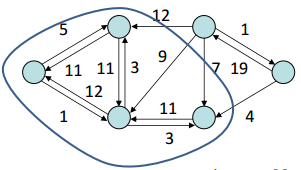
\includegraphics[scale=0.50]{slides.png}
  \caption{}
\end{figure}

Este resultado deve-se à sucessiva inversão de arestas $"$interiores$"$, até que a dado ponto seja impossível chegar desde a origem ao destino. Os nós $"$\textit{half discovered}$"$ serão os nós necessários para retirar para que o não seja descoberto nenhum caminho da origem para o destino.

Esta função contém também a terceira parte do projeto, em que nos é pedido para calcular a conetividade do grafo e fornecer os nós que separam o grafo. Esta parte de código encontra-se contemplada no \textit{if} final da função, em que, caso o número de nós que é necessário retirar para separar um nó de outro seja inferior ao número de nós da iteração anterior, atualiza-se a \textit{string} que contém os indentificadores desses nós, passando a conter apenas os que separaram o grafo nesta iteração. A conetividade é, simplesmente, o número mínimo de nós a retirar após corrido o programa para todos os pares de nós do grafo.

No que respeita à complexidade do algoritmo, tal como o algoritmo original, terá uma complexidade O(mf). No algoritmo original, \textit{m} representa as arestas do grafo e \textit{f} o fluxo máximo encontrado (para as inversões) que neste caso é unitário, ficando a complexidade simplificada para O(m).

\section{Função \textit{cumulative\_statistics}}
Esta função destina-se à segunda parte do projeto, em que é necessário calcular a distribuição cumulativa do número mínimo de nós a serem retirados. Não se irá apresentar pseudo-código dada a simplicidade da função.

Ao correr cada iteração da função \textit{ford\_fulkerson} é actualizado o vetor \textit{node\_statistics}, que é responsável pelo armazenamento do número de vezes que determinado número de nós é necessário retirar para separar dada origem e destino.

Quando o vetor fica com os valores finais relativos à rede dada no ficheiro, é calculado na função \textit{cumulative\_statistics} as ocorrências totais de cada número de nós a serem retirados. É, depois, impresso no terminal a divisão das ocorrências de cada índice do vetor pelo valor total das ocorrências, sendo omitida a posição 0 desse vetor. Esta posição representa o número de ocorrências em que se tentou obter o número de nós a retirar para separar dois nós diretamente ligados. 

%visto que as estatísticas de nenhum nó ser necessário retirar não é interessante para o projeto, apesar de %se ter em conta nas ocorrências totais.

\section{Considerações Finais}
Com a resolução deste mini-projeto conseguimos compreender melhor o algoritmo de \textit{Ford Fulkerson} que, apesar de adaptado, esteve bastante presente na nossa implementação, bem como algoritmos previamente estudados como a \textit{BFS (Breadth First Search)} e, finalmente, o teorema do \textit{max flow min cut}, dado recentemente nas aulas teóricas.

Para testar \textit{for correctness} o nosso código, utilizámos uma série de grafos, sendo os mais relevantes os apresentados nas figuras 1, 2, 3 e 4.

\begin{figure}[!htb]
\minipage{0.32\textwidth}
   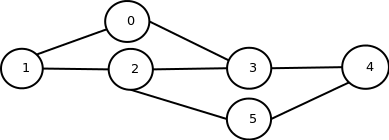
\includegraphics[width=\textwidth]{esquesito.png}
    \caption{É preciso tirar 2 nós (ex. tirar nós 1 e 3) para separar o grafo}
\endminipage\hfill
\minipage{0.32\textwidth}
   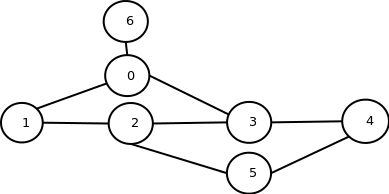
\includegraphics[width=\textwidth]{esquesito1.png}
    \caption{É preciso tirar só 1 nó (nó 0) para separar o grafo}
\endminipage\hfill
\minipage{0.32\textwidth}%
  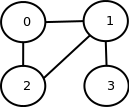
\includegraphics[scale=0.3]{grafo_pequeno.png}
  \caption{É preciso tirar só 1 nó (nó 1) para separar o grafo}
\endminipage
\end{figure}

Existem no entanto, algumas limitações do programa, especificadas no enunciado, como a existência de um máximo de 100 nós com índices entre 0 e 99. Assumimos também que não pode existir nó 1 se não existir nó 0, pois apesar de o programa correr corretamente e o número de nós a retirar ser correto, as estatísticas não irão ser as corretas, visto que o programa assume que existe uma ligação do nó 0, que está em falta no ficheiro de entrada, para todos os outros nós do grafo.

De forma a tornar o programa mais \textit{user friendly} criou-se um menu inicial em que o utilizador escolhe um de dois modos de funcionamento do programa:

\begin{enumerate}
	\item No primeiro modo o utilizador escolhe uma origem e um destino, existentes no grafo, o programa irá retornar o número de nós necessários para os separar e qual esse conjunto de nós.
	\item No segundo modo o utilizador não introduz quaisquer \textit{inputs}, o programa irá correr, automaticamente, para todos os pares de nós, calculando a distribuição cumulativa, o número mínimo de nós a retirar para que o grafo seja conexo e, finalmente, o conjunto dos nós a retirar para que tal aconteça.
\end{enumerate}

A complexidade geral do programa será assim, considerando o pior caso, O(n)[\textit{complexidade da função "init\_vector"}]+O(n\textsuperscript{2})[\textit{repetição de "ford\_folkerson$"$ para todos os pares de nós do grafo}]*O(m)[\textit{Complexidade da função "ford\_folkerson"}] +O(n) [\textit{Complexidade da função "cumulative\_statistics"}]. A complexidade final será entao O(mn\textsuperscript{2}), sendo \textit{m} o número de arestas e \textit{n} o número de nós.

\end{document}